\documentclass[11pt,a4paper,onecolumn,oneside,notitlepage]{article}
\usepackage[utf8]{inputenc}
\usepackage[english]{babel}
\usepackage{amsmath}
\usepackage{amsfonts}
\usepackage{amssymb}
\usepackage{graphicx}
\usepackage{bbm}
\usepackage[left=2cm,right=2cm,top=2cm,bottom=2cm]{geometry}

\usepackage[backend=biber, %% Hilfsprogramm "biber" (statt "biblatex" oder "bibtex")
style=authoryear, %% Zitierstil (siehe Dokumentation)
natbib=true, %% Bereitstellen von natbib-kompatiblen Zitierkommandos
hyperref=true, %% hyperref-Paket verwenden, um Links zu erstellen
]{biblatex}
\addbibresource{paper.bib}

\author{Mokrane Yahiatene\\
	\begin{small}
		Deep Learning for Natural Language Processing -- SS21 -- Philipp Cimiano and Philipp Heinisch
	\end{small}
}
\title{SemEval-2020 Task 7: Assessing Humor in Edited
	News Headlines - Subtask 2 (Funnier)}
\begin{document}
	\maketitle
	
	\section{Introduction}
		Humor is a communicative ability resulting in laughter and joy for humans. Assessing text based humor has peaked the interest of many researchers and has been a very challenging task in the Natural Language Processing field.
		The difficulties in assesing funniness lie in the subjective nature of humor. Humans have different tastes in humor and dependends of a lot of factors  f.e.: language,regionality, social status etc.
		Basically a lot of demographic aspects play an important part in finding soemthing humorous.
		If we manage to get good results in generating, detecting and grading humor it would be a huge progress in this scientific field. There would be also quite a few business application for humor assesing (f.e. humor text generating).
		SemEval-2020 Task 7 is a humor-grading task consisting of two subtask(subtask 1, subtask 2) with data from news headlines. These headlines got changed by replacing a single word/entity(micro changes) to make them funnier and afterwards being graded from scores between 0 and 3 , where 0 is the 'least funny' and 3 the 'most funny'.
		The first subtask consists of the originial headline and an edited headline where one must predict the funniness of the edited headline.
		The second subtask comprises of a classification task where one must predict the funnier headline when given the same headline  two times and replacing one entity in those headlines (originial1 ,edited1,originial2,edited2).
		This work tries to solve the second subtask with the help of a pretrained transformer model(BERT).
		
		
	\section{Related work}
		In this section we mainly look at the work \textcite{Bert1}
		They test the ability of BERT and its derivatives (RoBERTa, DistilBERT and ALBERT) in humor grading and classification tasks(subtask 1 and subtask 2) on the Humicroedit and the FunLines dataset.
		Their way of solving both tasks is to create a  BERT model and use the originial weights and  pre trained BERT model weights  fine tuned  with a masked language model layer on top.They compare both weigths' results. After that they put a regression layer on top to solve sub task 1 and then they use their model from sub task 1 to solve sub task 2 with zero shot inference. 
		To be precise they followed a masked language modeling approach on the entire dataset only using the edited texts as input while masking all the words in the text for prediction. They chose a maximum sequence length of 256 tokens for masked word prediction. They also experiment with the original BERT Model weights to initiliaze sub task 1 model weights and compare the results.
		Noteworthy is the fact that for sub  task 1 they fed the model the orignial headline and the edited text and for subtask 2 they concatenated the originial headline 1 with the edited headline 1 and concatenated the originial headline 2 with the edited headline 2 and fed the model 2 sentences.
		The reason for that is that the context between the originial end edited headline was deemed important.
		  \begin{figure}
			\begin{center}
				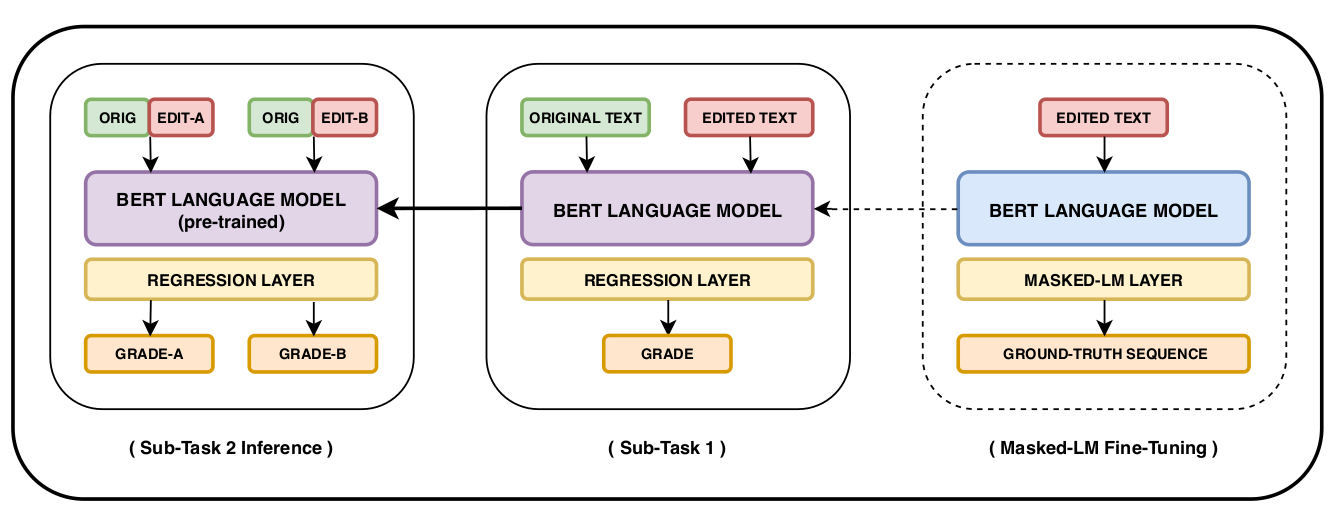
\includegraphics[width=1.0\linewidth]{system_architecture.png}
			\end{center}
			
			\caption{Model Architecture taken from \textcite{Bert1} }\label{fig1}
		\end{figure}	


	\section{Method}
		We have access to the humicroedit data set and an additionial funlines data set.
		For our approach we only used the humicroedit data set and split the data in 64\%(train) to 16\%(validation) to 20\% (test) fashion. The data is split into 10 columns although for us the most relevant are the following: originial1,edit1,meanGrade1,originial2,edit2,meanGrade2,label.
		The originial1 and original2 are the same headline but  only differ by the word which gets replaced while edit1 and edit2 are two different entities which will replace those words in original1 and original2. The label tells us which edited headline is funnier by using the meanGrade1 and meanGrade2 column.´
		In this section I use a different approach: similiar to above mentioned approach I concatenated originial headlines with edited headlines but instead of generating 2 sentences I concatenate them again to one sentence in following manner: originial1 + edited1 + originial2 + edited2.
		This new sentence is fed as input into my model which is shown in figure 3.
		My model differs from the usual approach seen in the competition(regression task for task 1 and task 2), instead I'm trying a multi class classification approach with 3 classes. Namely 0,1,2 with the meaning "0": both edited headlines are equally funny, "1" first headline is funnier than second and "2" second headline is funnier than first.
		I chose a sequence length of 256 and a batch size of 8 for all my data sets (train,dev,test) with two input layers for the input ids and the attention mask.
		Between the BERT layer and my final output layer I put a Dropout layer of size 1024 for better generalization which gave slightly better results. 
		Finally I added a last output layer with a softmax activation function over 3 output classes.
		%TODO: give some reasons [avantages] why you go with your assigned language model
	
	    \begin{figure}
		\begin{center}
			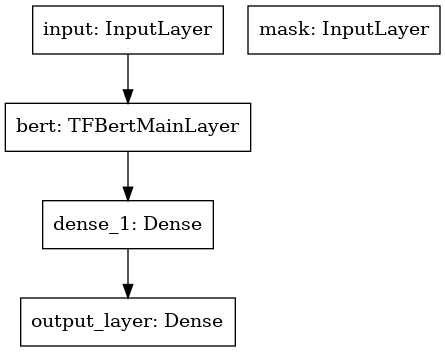
\includegraphics[width=1.0\linewidth]{model.png}
		\end{center}
		
		\caption{Model Architecture}\label{fig3}
	\end{figure}	
		
	\section{Evaluation}
    In this section we want to see how our own model and approach fares against the other participants in the competition especially against the model by \textcite{Bert1} using the pretrained BERT model .
    I tested my approach with 3 different sizes of the BERT model namely bert-base-cased, bert-base-uncased, bert-large-uncased and evaluated those models on my test set. In the competition there are 2 different metrics for evaluating sub task 2: Accuracy and Reward where reward wasn't used for ranking. See \textcite{Bert2}\\\\
    Accuracy= $\frac{C}{N}$\\\\
    Reward= $\frac{1}{N} \Sigma_{i=1}^N(\mathbbm{1}_{\hat{y}_i = y_i}- \mathbbm{1}_{\hat{y}_i \neq y_i}    ) f_i^{(1)} - f_i^{(2)} $\\\\
    For that reason we use accuracy for grading and comparing our results.
    
		
		\begin{table}
			\begin{center}
				\begin{tabular}{|c|c|}
					\hline
					\textbf{Model} &  \textbf{Accuracy}\\
					\hline
					\hline
					BERT base cased & \textbf{0.45}\\
					\hline
					BERT base uncased & \textbf{0.48}\\
					\hline
					BERT large uncased & \textbf{0.46}\\
					\hline
				\end{tabular}
			\end{center}
			
			\caption{Results}\label{tab1}
		\end{table}				
		
	    \begin{figure}
	\begin{center}
		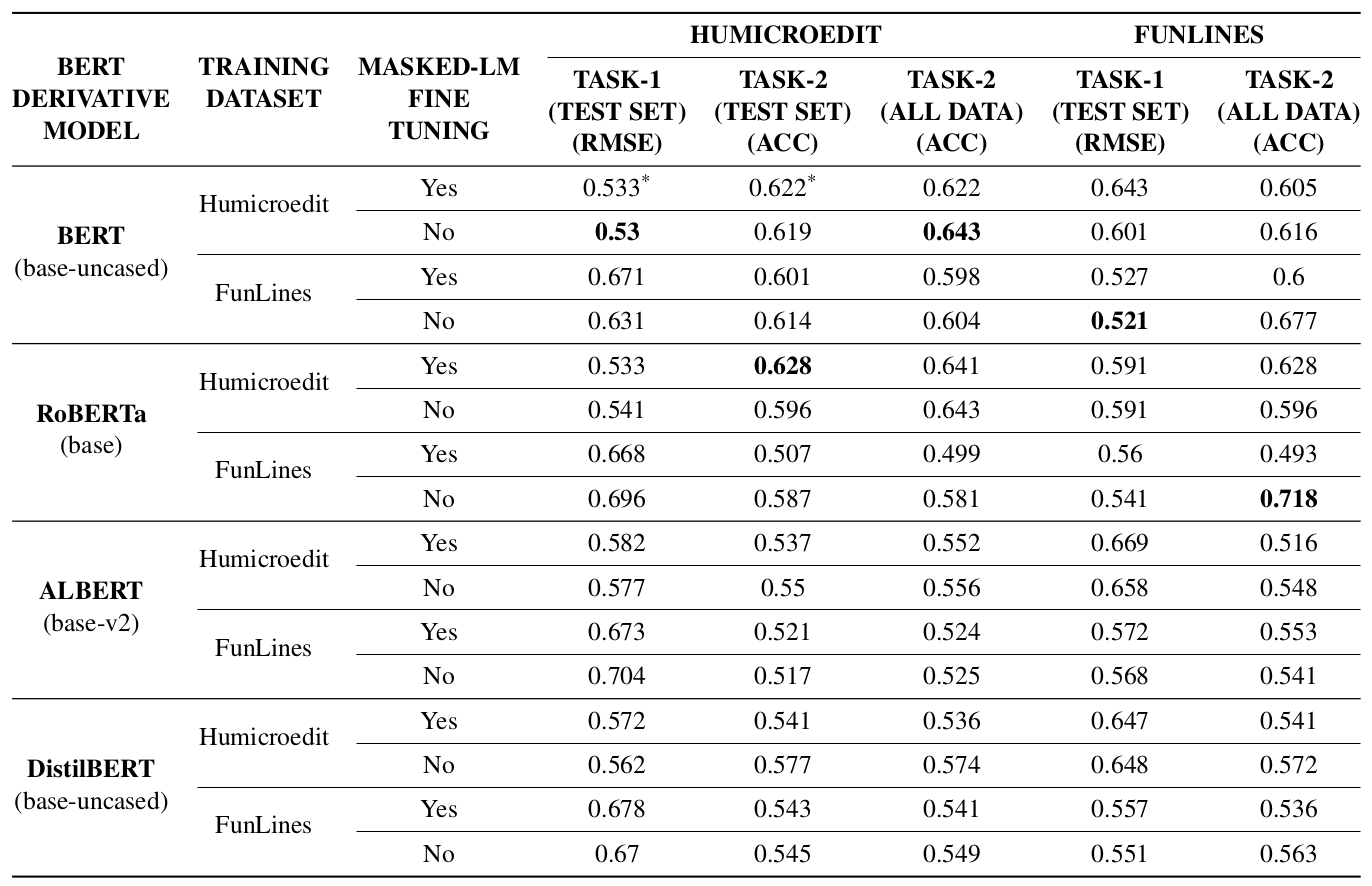
\includegraphics[width=1.0\linewidth]{eval_table.png}
	\end{center}
	
	\caption{Evaluation scores taken from \textcite{Bert1}}\label{fig4}
\end{figure}	
	\section{Conclusion}
	In this work we tested the ability of the pretrained BERT Model for state of the art NLP tasks to be precise assesing humor in edited headlines. With little effort one can achieve relatively good results on a custom fine tuned model.  Almost every competitor used their model architecture from sub task 1 and used it for sub task 2 with zero shot inference. Those who didnt choose this approach had significantly lower results. Also picking the right pretrained model had quite an influence on the results . Score wise we can see that RoBERTa seems to be leading closely followed by BERT.   We have seen that state of the art approaches  only achieve medicore results compared to other NLP tasks (Rank 1 : Team Hitachi on RoBERTa, task 1: RMSE: 0.522 , task 2: Accuracy: 0.65). This shows humor related NLP tasks still need a lot more research and work done.
	Future work could include experimenting with different pretrained models, trying new language model techiques or different approaches in customizing the input.
	\printbibliography
\end{document}